\section{Function arguments statistics}
\label{args_stat}

I've always been interesting in what is average number of function arguments.

\index{UNIX!grep}
Just analysed many Windows 7 32-bit DLLs \\
(crypt32.dll, mfc71.dll, msvcr100.dll, shell32.dll, 
user32.dll, d3d11.dll, mshtml.dll, msxml6.dll, sqlncli11.dll, wininet.dll, mfc120.dll, msvbvm60.dll, ole32.dll, themeui.dll, wmp.dll) 
(because they use stdcall convention, and so it is to grep disassembly output just by \INS{RETN X}).

\begin{itemize}
\item no arguments: ~29\%
\item 1 argument: ~23\%
\item 2 arguments: ~20\%
\item 3 arguments: ~11\%
\item 4 arguments: ~7\%
\item 5 arguments: ~3\%
\item 6 arguments: ~2\%
\item 7 arguments: ~1\%
\end{itemize}

\begin{figure}[H]
\centering
\ifdefined\ebook
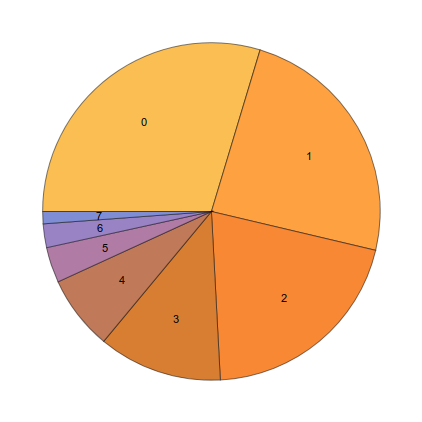
\includegraphics[width=0.7\textwidth]{other/args_stat.png}
\else
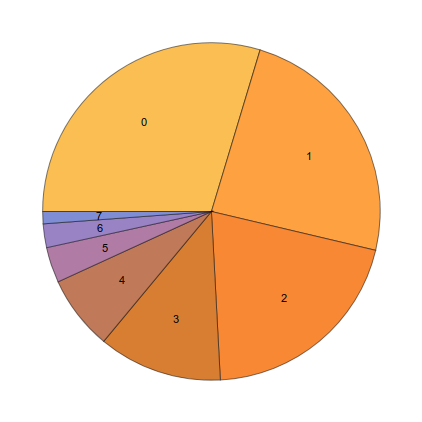
\includegraphics[width=0.5\textwidth]{other/args_stat.png}
\fi
\caption{Function arguments statistics}
\end{figure}

This is heavily dependent on programming style and may be very different for other software products.

